\documentclass[fleqn, a4paper, 11pt, oneside]{amsart}
%\usepackage[top = 2cm, bottom = 1cm, left = 1cm, right = 1cm]{geometry}
\usepackage{exsheets, tasks}
\usepackage{amsmath, amssymb, amsthm} %standard AMS packages
\usepackage{marginnote} %marginnotes
\usepackage{gensymb} %miscellaneous symbols
\usepackage{commath} %differential symbols
\usepackage{xcolor} %colours
\usepackage{cancel} %cancelling terms
\usepackage[free-standing-units, space-before-unit]{siunitx} %formatting units
\usepackage{tikz, pgfplots} %diagrams
\usetikzlibrary{calc, hobby, patterns, intersections, decorations.markings}
\usepackage{graphicx} %inserting graphics
\usepackage{hyperref} %hyperlinks
\usepackage{datetime} %date and time
\usepackage{ulem} %underline for \emph{}
\usepackage{xfrac} %inline fractions
\usepackage{enumerate,enumitem} %numbered lists
\usepackage{float} %inserting floats
\usepackage{circuitikz}[american voltages, american currents] %circuit diagrams
\usepackage[utf8]{inputenc}

\newcommand\numberthis{\addtocounter{equation}{1}\tag{\theequation}} %adds numbers to specific equations in non-numbered list of equations

\newcommand{\AxisRotator}[1][rotate=0]{
	\tikz [x=0.25cm,y=0.60cm,line width=.2ex,-stealth,#1] \draw (0,0) arc (-150:150:1 and 1);%
} %rotation symbols on axes

\theoremstyle{definition}
\newtheorem{example}{Example}
\newtheorem{definition}{Definition}

\theoremstyle{theorem}
\newtheorem{theorem}{Theorem}

\newcommand{\curl}{\mathrm{curl\,}}

\makeatletter
\@addtoreset{section}{part} %resets section numbers in new part
\makeatother

\renewcommand{\thesubsection}{(\arabic{subsection})}
\renewcommand{\thesection}{(\arabic{section})}

%section headings on left
\makeatletter
\def\specialsection{\@startsection{section}{1}%
	\z@{\linespacing\@plus\linespacing}{.5\linespacing}%
	%  {\normalfont\centering}}% DELETED
	{\normalfont}}% NEW
\def\section{\@startsection{section}{1}%
	\z@{.7\linespacing\@plus\linespacing}{.5\linespacing}%
	%  {\normalfont\scshape\centering}}% DELETED
	{\normalfont\scshape}}% NEW
\makeatother

%forces newline after subsection
\makeatletter
\def\subsection{\@startsection{subsection}{3}%
	\z@{.5\linespacing\@plus.7\linespacing}{.1\linespacing}%
	{\normalfont\itshape}}
\makeatother

\settasks{counter-format = tsk[1].}

\SetupExSheets{solution/print = true}

%opening
\title{Quantum and Solid State Physics : Assignment 2}
\author
{
	Aakash Jog\\
	ID : 989323563
}
\date{\formatdate{29}{10}{2015}}

\begin{document}

\tikzset{->-/.style={decoration={
  markings,
  mark=at position #1 with {\arrow{>}}},postaction={decorate}}}

\maketitle
%\setlength{\mathindent}{0pt}

\begin{question}
	Treating atoms as hard spheres that are as densely packed as possible, calculate the fraction of the unit cell volume filled with hard spheres, i.e. the atomic packing factor, for
	\begin{enumerate}
		\item SC
		\item BCC
		\item FCC
		\item Diamond
	\end{enumerate}
	Draw the unit cell for each of the above structures.
\end{question}

\begin{solution}
	\begin{enumerate}[leftmargin=*]
		\item
			Let the lattice constant be $a$.\\
			Therefore the radius of each atom is $\frac{a}{2}$.\\
			The total number of atoms in a unit cell of SC is $1$.\\
			Therefore,
			\begin{align*}
				\text{APF} & = \frac{\frac{4}{3} \pi \left( \frac{a}{2} \right)^3}{a^3} \\
                                           & = \frac{\frac{4}{3} \pi \frac{a^3}{8}}{a^3}                \\
                                           & = \frac{\pi}{6}
			\end{align*}
		\item
			Let the lattice constant be $a$.\\
			Therefore the radius of each atom is $\frac{a \sqrt{3}}{4}$.\\
			The total number of atoms in a unit cell of BCC is $2$.\\
			Therefore,
			\begin{align*}
				\text{APF} & = \frac{2 \cdot \frac{4}{3} \pi \left( \frac{a \sqrt{3}}{4} \right)^3}{a^3} \\
                                           & = \frac{\frac{8}{3} \pi \frac{3 \sqrt{3} a^3}{16}}{a^3}                     \\
                                           & = \frac{\sqrt{3} \pi}{2}
			\end{align*}
		\item
			Let the lattice constant be $a$.\\
			Therefore the radius of each atom is $\frac{a \sqrt{2}}{4}$.\\
			The total number of atoms in a unit cell of FCC is $2$.\\
			Therefore,
			\begin{align*}
				\text{APF} & = \frac{4 \cdot \frac{4}{3} \pi \left( \frac{a \sqrt{2}}{4} \right)^3}{a^3} \\
                                           & = \frac{\frac{16}{3} \pi \frac{2 \sqrt{2} a^3}{16}}{a^3}                    \\
                                           & = \frac{2 \sqrt{2} \pi}{3}
			\end{align*}
		\item
			Let the lattice constant be $a$.\\
			Therefore the radius of each atom is $\frac{a \sqrt{3}}{8}$.\\
			The total number of atoms in a unit cell of diamond lattice is $8$.\\
			Therefore,
			\begin{align*}
				\text{APF} & = \frac{8 \cdot \frac{4}{3} \pi \left( \frac{a \sqrt{3}}{8} \right)^3}{a^3} \\
                                           & = \frac{\frac{32}{3} \pi \frac{3 \sqrt{3} a^3}{512}}{a^3}                   \\
                                           & = \frac{\sqrt{3} \pi}{16}
			\end{align*}
	\end{enumerate}
\end{solution}

\begin{question}
	Please refer to the following figure, which shows the relationship between the energy band gap, and lattice constants for several materials.
	\begin{figure}[H]
		\centering
		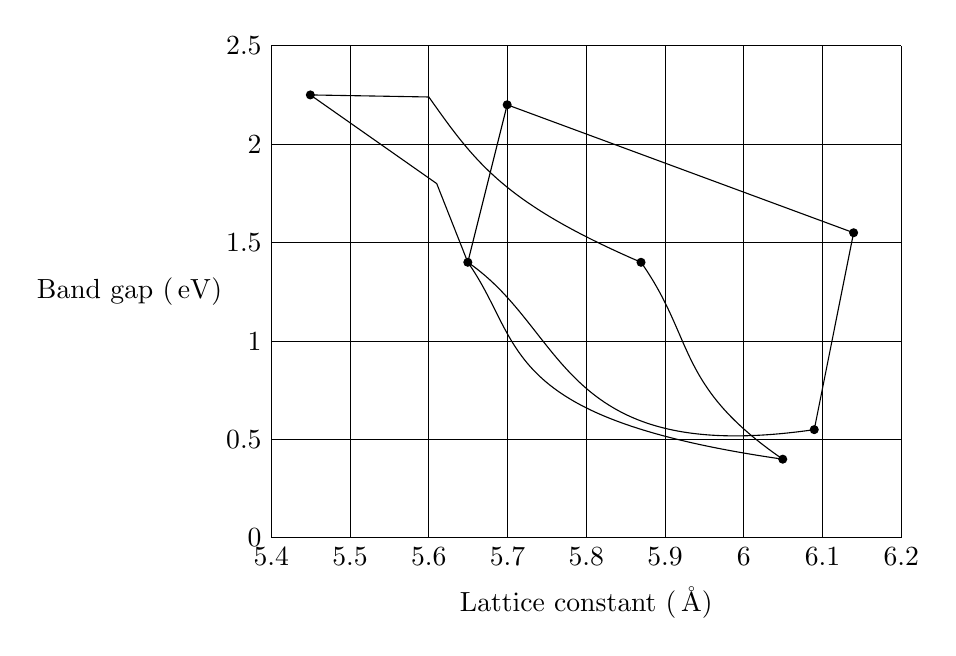
\begin{tikzpicture}[xscale = 10, yscale = 2.5]
			\begin{scope}
				\foreach \x in {5.4,5.5,5.6,5.7,5.8,5.9,6,6.1,6.2}
				{
					\draw (\x,0) node [below] {$\x$} -- (\x,2.5);
				}

				\foreach \y in {0,0.5,1,1.5,2,2.5}
				{
					\draw (5.4,\y) node [left] {$\y$} -- (6.2,\y);
				}
			\end{scope}

			\begin{scope}
				\node [left, xshift = -0.5cm] at (5.4,1.25) {Band gap (\electronvolt)};
				\node [below, yshift = -0.5cm] at (5.8,0) {Lattice constant (\angstrom)};
			\end{scope}

			\coordinate (GaP) at (5.45,2.25);
			\coordinate (GaAs) at (5.65,1.4);
			\coordinate (AlAs) at (5.7,2.2);
			\coordinate (InP) at (5.87,1.4);
			\coordinate (InAs) at (6.05,0.4);
			\coordinate (GaSb) at (6.09,0.55);
			\coordinate (AlSb) at (6.14,1.55);

			\begin{scope}
				\draw (GaP) to (5.6,2.24) [out = 280, in = 120] to (InP);
				\draw (InP) to [out = 280, in = 110] (InAs);
				\draw (GaP) to (5.61,1.8) to (GaAs) to [out = 280, in = 150] (InAs);
				\draw (GaAs) to (AlAs) to (AlSb) to (GaSb);
				\draw (GaAs) to [out = 290, in = 210] (GaSb);
			\end{scope}

			\begin{scope}
				\filldraw (GaP) circle [x radius = 0.05mm, y radius = 0.2mm];
				\filldraw (GaAs) circle [x radius = 0.05mm, y radius = 0.2mm];
				\filldraw (AlAs) circle [x radius = 0.05mm, y radius = 0.2mm];
				\filldraw (InP) circle [x radius = 0.05mm, y radius = 0.2mm];
				\filldraw (InAs) circle [x radius = 0.05mm, y radius = 0.2mm];
				\filldraw (GaSb) circle [x radius = 0.05mm, y radius = 0.2mm];
				\filldraw (AlSb) circle [x radius = 0.05mm, y radius = 0.2mm];
			\end{scope}
		\end{tikzpicture}
	\end{figure}
	\begin{enumerate}
		\item
			Consider growing an epitaxial later of InAs on the following substrates
			\begin{enumerate}
				\item InP
				\item AlAs
				\item GaAs
				\item GaP
			\end{enumerate}
			For which substrate would there be minimum strain in the growth structure, and why?
			\begin{enumerate}
				\item InP
				\item AlAs
				\item GaAs
				\item GaP
			\end{enumerate}
		\item
			Draw a line on the figure above, such that all materials along this line could be grown as lattice-matched epitaxial layers to an underlying InP substrate.
	\end{enumerate}
\end{question}

\begin{solution}
	\begin{enumerate}[leftmargin=*]
		\item
			There would be minimum strain in the growth structure if the substrate used is InP.
			This is because the difference between the lattice constants of InAs and InP, as compared to the other alternatives.
		\item
			\begin{figure}[H]
				\centering
				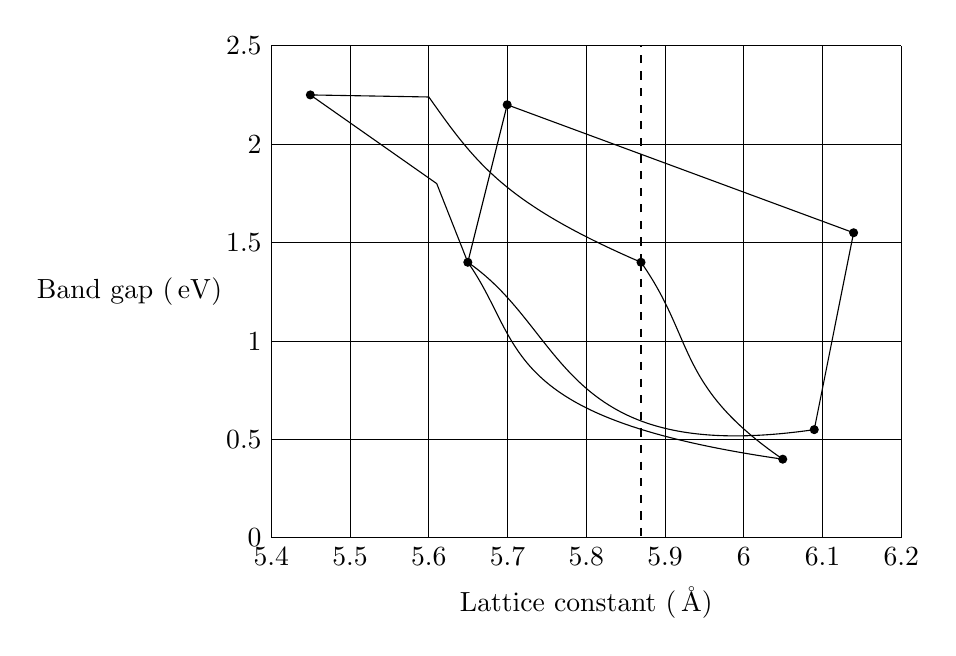
\begin{tikzpicture}[xscale = 10, yscale = 2.5]
					\begin{scope}
						\foreach \x in {5.4,5.5,5.6,5.7,5.8,5.9,6,6.1,6.2}
						{
							\draw (\x,0) node [below] {$\x$} -- (\x,2.5);
						}

						\foreach \y in {0,0.5,1,1.5,2,2.5}
						{
							\draw (5.4,\y) node [left] {$\y$} -- (6.2,\y);
						}
					\end{scope}

					\begin{scope}
						\node [left, xshift = -0.5cm] at (5.4,1.25) {Band gap (\electronvolt)};
						\node [below, yshift = -0.5cm] at (5.8,0) {Lattice constant (\angstrom)};
					\end{scope}

					\coordinate (GaP) at (5.45,2.25);
					\coordinate (GaAs) at (5.65,1.4);
					\coordinate (AlAs) at (5.7,2.2);
					\coordinate (InP) at (5.87,1.4);
					\coordinate (InAs) at (6.05,0.4);
					\coordinate (GaSb) at (6.09,0.55);
					\coordinate (AlSb) at (6.14,1.55);

					\begin{scope}
						\draw (GaP) to (5.6,2.24) [out = 280, in = 120] to (InP);
						\draw (InP) to [out = 280, in = 110] (InAs);
						\draw (GaP) to (5.61,1.8) to (GaAs) to [out = 280, in = 150] (InAs);
						\draw (GaAs) to (AlAs) to (AlSb) to (GaSb);
						\draw (GaAs) to [out = 290, in = 210] (GaSb);
					\end{scope}

					\begin{scope}
						\filldraw (GaP) circle [x radius = 0.05mm, y radius = 0.2mm];
						\filldraw (GaAs) circle [x radius = 0.05mm, y radius = 0.2mm];
						\filldraw (AlAs) circle [x radius = 0.05mm, y radius = 0.2mm];
						\filldraw (InP) circle [x radius = 0.05mm, y radius = 0.2mm];
						\filldraw (InAs) circle [x radius = 0.05mm, y radius = 0.2mm];
						\filldraw (GaSb) circle [x radius = 0.05mm, y radius = 0.2mm];
						\filldraw (AlSb) circle [x radius = 0.05mm, y radius = 0.2mm];
					\end{scope}

					\begin{scope}
						\draw [dashed] (InP) -- ++(-90:1.4);
						\draw [dashed] (InP) -- ++(90:1.1);
					\end{scope}
				\end{tikzpicture}
			\end{figure}
	\end{enumerate}
\end{solution}

\begin{question}
	Determine whether the following statements are true or false, and explain your answer.
	\begin{enumerate}
		\item
			The wavelength of the electron is given by the de Broglie equation.
		\item
			The wave associated with a moving electron is an electromagnetic wave.
		\item
			The kinetic energy of the electron is given by the equation $E = h f$.
		\item
			A photograph of a person is created with only a few incident photons, and the output image collected on a screen.
			The result of this experiment is a very faint image of the person.
		\item
			The solution to the Schrödinger equation is the wave function, which is a probability amplitude of a quantum system in space and time.
	\end{enumerate}
\end{question}

\begin{solution}
	\begin{enumerate}[leftmargin=*]
		\item
			True, according to the de Broglie hypothesis, the wavelength of a wave corresponding to a particle is given by the de Broglie equation.
		\item
			False, the wave associated with a moving electron is not an electromagnetic wave, but is an hypothetical wave which describes the wave function $\psi$.
		\item
			False, the equation $E = h f$ gives the total, i.e. kinetic and potential energy of the electron.
		\item
			False, the result of this experiment is a few dots on the screen, as the interaction of the photons with the person forces them to behave like particles.
		\item
			False, the solution is the wave function, which is a complex number, whose square is the probability amplitude of a quantum system in space and time.
	\end{enumerate}
\end{solution}

\begin{question}
	Suppose you drop a rock off a cliff of a height $h$.
	As it falls, a million photographs are taken, at random intervals.
	On each picture, the distance of the rock has fallen is being measured.
	\begin{enumerate}
		\item
			Show that the probability density is given by
			\begin{align*}
				\rho(x) & = \frac{1}{2 \sqrt{h x}}
			\end{align*}
			where $0 \le x \le h$.
		\item
			What is the average of all measured distances?
		\item
			what is the standard deviation for the measured distances?
		\item
			What is the probability that a photograph, selected at random, would show a distance $x$ more than one standard deviation away from the average?
	\end{enumerate}
\end{question}

\begin{solution}
	\begin{enumerate}[leftmargin=*]
		\item
			\begin{align*}
				x(t) & = \frac{1}{2} g t^2
			\end{align*}
			Let the total time of the free fall be $T$.\\
			Therefore,
			\begin{align*}
				T & = \sqrt{\frac{2 h}{g}}
			\end{align*}
			Therefore,
			\begin{align*}
				P \frac{\dif t}{T} & = \frac{\dif x}{\sqrt{\frac{2 h}{g}} g \sqrt{\frac{2 x}{g}}} \\
                                                   & = \frac{\dif x}{2 \sqrt{h x}}
			\end{align*}
			As the rock is falling under constanct acceleration,
			\begin{align*}
				\dod{x}{t} & = g t
			\end{align*}
			Therefore,
			\begin{align*}
				\rho(x) & = \frac{1}{2 \sqrt{h x}}
			\end{align*}
		\item
			\begin{align*}
				\langle x \rangle & = \int\limits_{0}^{h} x \rho(x)                             \\
                                                  & = \int\limits_{0}^{h} \frac{x \dif x}{2 \sqrt{h x}}         \\
                                                  & = \int\limits_{0}^{h} \frac{\sqrt{x}}{2 \sqrt{h}} \dif x    \\
                                                  & = \left. \frac{x^{\frac{3}{2}}}{3 \sqrt{h}} \right|_{0}^{h} \\
                                                  & = \frac{h^{\frac{3}{2}}}{3 h^{\frac{1}{2}}}                 \\
                                                  & = \frac{h}{3}
			\end{align*}
		\item
			\begin{align*}
				\sigma^2          & = \int\limits_{0}^{h} x^2 \rho(x) \dif x - \left( \int\limits_{0}^{h} x \rho(x) \dif x \right)           \\
                                                  & = \int\limits_{0}^{h} \frac{x^2}{2 \sqrt{h x}} \dif x - \frac{h^2}{9}                                    \\
                                                  & = \left. \frac{1}{2 \sqrt{h}} \left( \frac{2}{5} x^{\frac{5}{2}} \right) \right|_{0}^{h} - \frac{h^2}{9} \\
                                                  & = \frac{h^2}{5} - \frac{h^2}{9}                                                                          \\
                                                  & = \frac{4 h^2}{45}                                                                                       \\
				\therefore \sigma & = \frac{2 h}{3 \sqrt{5}}
			\end{align*}
		\item
			\begin{align*}
				\sigma & = \frac{2 h}{3 \sqrt{5}}
			\end{align*}
			Therefore,
			\begin{align*}
				\langle x \rangle - \sigma + x & = \frac{h}{3} - \frac{2 h}{3 \sqrt{5}} + x \\
                                                               & = \frac{h (\sqrt{5} - 2)}{3 \sqrt{5}} + x  \\
				\langle x \rangle + \sigma + x & = \frac{h}{3} - \frac{2 h}{3 \sqrt{5}} + x \\
                                                               & = \frac{h (\sqrt{5} + 2)}{3 \sqrt{5}} + x
			\end{align*}
			Therefore,
			\begin{align*}
				\rho\left( \langle x \rangle - \sigma + x \right) & = \rho\left( \frac{h (\sqrt{5} + 2)}{3 \sqrt{5}} + h x \right)   \\
                                                                                  & = \frac{1}{2 \sqrt{h \frac{h (\sqrt{5} - 2)}{3 \sqrt{5}} + h x}} \\
                                                                                  & = \frac{1}{2 \sqrt{\frac{h^2 (\sqrt{5} - 2)}{3 \sqrt{5}} + h x}} \\
				\rho\left( \langle x \rangle + \sigma + x \right) & = \rho\left( \frac{h (\sqrt{5} + 2)}{3 \sqrt{5}} + h x \right)   \\
                                                                                  & = \frac{1}{2 \sqrt{h \frac{h (\sqrt{5} + 2)}{3 \sqrt{5}} + h x}} \\
                                                                                  & = \frac{1}{2 \sqrt{\frac{h^2 (\sqrt{5} + 2)}{3 \sqrt{5}} + h x}} \\
			\end{align*}
	\end{enumerate}
\end{solution}

\end{document}
